\documentclass[a4,12pt]{amsart}

\newcounter{chapter}% HACK since amsart has no chapter counter like amsbook
%and there is \numberwithin{theorem}{chapter} in macros.tex,
%seemingly overruled by \numberwithin{theorem}{section} in top.tex

\input macros
\begin{document}
\input topZTors

\section{The integers}
\label{sec:integers}

We define the type of integers in one of the many possible ways.

\begin{definition}\label{def:integers}
Let $\zet$ be the inductive type with the following three constructors:
\begin{enumerate}
\item $\zzero: \zet$ for the integer number zero, 
$0 \defeq \zzero$
\item $\zpos: \NN \to \zet$ for positive numbers,
$1 \defeq \zpos(0),\ldots$.
\item $\zneg: \NN \to \zet$ for negative numbers, 
$-1 \defeq \zneg(0),\ldots$
\end{enumerate}

The \emph{embedding} function $i:\NN\to\zet$ is defined by induction,
setting $i(0)\defeq \zzero$, $i(S(n))\defeq \zpos(n)$.
Like the type $\NN$, the type $\zet$ is a set with decidable equality
and ordering relations,
and we denote its elements often in the usual way as $\ldots,-1,0,1,\ldots$.

One well-known equivalence is \emph{negation} ${-}:\zet\to\zet$, 
also called \emph{complement}, inductively defined by setting 
$-\zzero\defeq \zzero$, 
$-\zpos(n)\defeq \zneg(n)$, 
$-\zneg(n)\defeq \zpos(n)$.
Negation is its own inverse.

The \emph{successor} function $s:\zet\to\zet$ is defined inductively setting 
$s(\zzero)\defeq \zpos(0)$, 
$s(\zpos(n))\defeq \zpos(S(n))$,
$s(\zneg(n))\defeq -i(n)$. For example, we have
$s(-1)\jdeq s(\zneg(0))\jdeq -i(0) \jdeq \zzero \jdeq 0$.
By induction on $n:\NN$ one proves $s(i(n))=i(S(n))$, 
so that one can say that $s$ extends $S$
on the $i$-image of $\NN$. 

The successor function $s$ is an equivalence.
It is instructive to depict iterating $s$ in both directions as 
a doubly infinite sequence containing all integers:
\[
\ldots \mapsto \zneg(1) \mapsto \zneg(0) \mapsto \zzero \mapsto \zpos(0) \mapsto \zpos(1) \mapsto \ldots
\]

The inverse $s^{-1}$ of $s$ is called the \emph{predecessor} function.
We denote the $n$-fold iteration of $s$ as $s^n$, and
the $n$-fold iteration of $s^{-1}$ as $s^{-n}$.

Addition of integers is defined inductively by setting
$z + \zzero\defeq z$, 
$z + \zpos(n)\defeq s^{n+1}(z)$, 
$z + \zneg(n)\defeq s^{-(n+1)}(z)$.
Again, addition extends $+$ on the $i$-image of $\NN$,
see \cref{xca:addition-on-Z-and-N}. 
From addition and unary $-$ one can define a binary
\emph{substraction} function setting $z-y \defeq z+(-y)$.
\end{definition}

\begin{xca}\label{xca:addition-on-Z-and-N}
Show that $i(n+m)=i(n)+i(m)$ for all $n,m:\NN$.
\end{xca}


\section{Some induction principles for the integers}
\label{sec:integers-induction}

From the definition of $\zet$ we get the following slightly better induction principle:
Given $P : \zet \to \UU$, to construct an element of $P(z)$ for every $z : \zet$,
it suffices to give $P(0)$ and two functions
$f : \prod_{n:\NN}(P(n) \to P(n+1))$ and
$g : \prod_{n:\NN}(P(-n) \to P(-n-1))$,
see \cref{fig:integers-induction-asymmetric}.

\begin{figure}
  \centering
  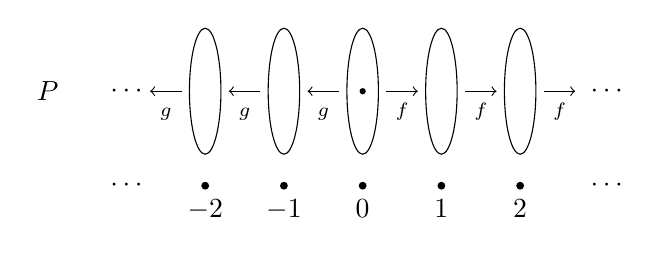
\begin{tikzpicture}
    \foreach \x in {-2,-1,0,1,2} {
      \begin{scope}[shift={(\x,0)}]
        \draw (0,0) ellipse (0.2 and 0.8);
        \node[fill,circle,inner sep=1pt,label=below:{$\x$}] (P\x) at (0,-1.2) {};
      \end{scope}
    }
    \foreach \x in {0,1,2} {
      \begin{scope}[shift={(\x,0)}]
        \draw[->] (0.3,0) -- node[below] {\scriptsize$f\strut$} (0.7,00);
      \end{scope}
    }
    \foreach \x in {-3,-2,-1} {
      \begin{scope}[shift={(\x,0)}]
        \draw[->] (0.7,0) -- node[below] {\scriptsize$g\strut$} (0.3,00);
      \end{scope}
    }
    \node[fill,circle,inner sep=.8pt] at (0,0) {};
    \node at (-4,0) {$P$};
    \node at (-4,-1.4) {$\ZZ$};
    \foreach \x in {-3,3.1} {
      \foreach \y in {0,-1.2} {
        \node at (\x,\y) {$\cdots$};
      }
    }
  \end{tikzpicture}
  \caption{Asymmetric integer induction principle}
  \label{fig:integers-induction-asymmetric}
\end{figure}

\begin{figure}
  \centering
  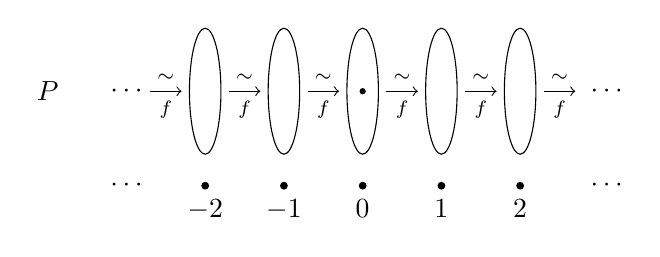
\begin{tikzpicture}
    \foreach \x in {-2,-1,0,1,2} {
      \begin{scope}[shift={(\x,0)}]
        \draw (0,0) ellipse (0.2 and 0.8);
        \node[fill,circle,inner sep=1pt,label=below:{$\x$}] (P\x) at (0,-1.2) {};
      \end{scope}
    }
    \foreach \x in {-3,-2,-1,0,1,2} {
      \begin{scope}[shift={(\x,0)}]
        \draw[->] (0.3,0) -- node[above] {\scriptsize$\sim$} node[below] {\scriptsize$f$} (0.7,00);
      \end{scope}
    }
    \node[fill,circle,inner sep=.8pt] at (0,0) {};
    \node at (-4,0) {$P$};
    \node at (-4,-1.4) {$\ZZ$};
    \foreach \x in {-3,3.1} {
      \foreach \y in {0,-1.2} {
        \node at (\x,\y) {$\cdots$};
      }
    }
  \end{tikzpicture}
  \caption{Symmetric integer induction principle}
  \label{fig:integers-induction-symmetric}
\end{figure}

\begin{figure}
  \centering
  \begin{tikzpicture}
    \foreach \x in {-2,-1,0,1,2} {
      \begin{scope}[shift={(2*\x,0)}]
      
        \node[fill,circle,inner sep=1pt,label=below:{$\x$}] (P\x) at (0,-1.2) {};
      \end{scope}
    }
    \foreach \x in {-3,-2,-1,0,1,2} {
      \begin{scope}[shift={(2*\x,0)}]
        \draw[->] (0.6,0) -- node[above] {\scriptsize$f_{\x}$} (1.3,00);
      \end{scope}
    }
    \node at (-4,0) {\scriptsize$h_- (1)$};
    \node at (-2,0) {\scriptsize$h_- (0)$};
    \node at (0,0) {\scriptsize$h_0$};
    \node at (2,0) {\scriptsize$h_+ (0)$};
    \node at (4,0) {\scriptsize$h_+ (1)$};
  %  \node at (-8,0) {$h$};
  %  \node at (-8,-1.4) {$\ZZ$};
    \foreach \x in {-6,6} {
      \foreach \y in {0,-1.3} {
        \node at (\x,\y) {$\cdots$};
      }
    }
  \end{tikzpicture}
  \caption{Bookkeeping $h=(h_-,h_0,h_+)$ OMIT WHEN OBSOLETE}
  \label{fig:bookkeeping-h-h0h+}
\end{figure}

It's possible to give a more symmetric, but less general induction principle,
if assume that the functions are equivalences.
In that case we can reorient the $g$'s to point in the same direction as the $f$'s,
so that we just give $f : \prod_{z:\zet}P(z) \equiv P(z+1)$, 
see \cref{fig:integers-induction-symmetric}.

We shall need that in this case, giving a element $h:\prod_{z:\zet}P(z)$
such that $h(z+1) = f_z(h(z))$ for all $z:\zet$
is in fact equivalent to giving the single element $h(0)$.
We formulate this precisely as follows.

\begin{theorem}\label{thm:integers-univ-symm}
  Let $P : \zet \to \UU$ and $f : \prod_{z:\zet}P(z) \equiv P(z+1)$. The function
  \[
    \varphi : \biggl(\sum_{h:\prod_{z:\zet}P(z)}\prod_{z:\zet}h(z+1) = f_z(h(z))\biggr) \to P(0)
  \]
  that sends $(h,q)$ to $h(0)$ is an equivalence.
\end{theorem}
\begin{proof}
  We prove that the fiber over any $p : P(0)$ is contractible.
  We simplify notations a bit by leaving out the types of $h$ and $q$.
  The fiber $\sum_{(h,q)} h(0)=p$ consists of a triples $(h,q,r)$ with $r : h(0) = p$.
  By case distinction, $h$ can (equivalently) be split in three parts $(h_-,h_0,h_+)$
  with $h_0 : P(0)$, $h_+ : \prod_{n:\NN}P(n+1)$,  and $h_- : \prod_{n:\NN} P(-n-1)$. 
  Since $h(0)=p$ only depends on $h_0$ the pair $(h_0,r)$ with  $r : h_0 = p$
  contracts away, so we're left with the type
  \begin{align*}
    \varphi^{-1}(p)
    &\equiv
      \Biggl(\sum_{h_+ : \prod_{n:\NN}P(n+1)}
      \bigl(h_+(0) = f_0(p)\bigr) \\
    &\qquad\qquad\qquad
      \times \biggl(\prod_{n:\NN}h_+(n+1) = f_n(h_+(n))\biggr)\Biggr) \\
    &\quad\times
      \Biggl(\sum_{h_- : \prod_{n:\NN}P(-n-1)}
      \bigl(h_-(0) = f_{-1}^{-1}(p)\bigr) \\
    &\qquad\qquad\qquad
      \times \biggl(\prod_{n:\NN}h_-(n+1) = f_{-n-2}^{-1}(h_-(n))\biggr)\Biggr).
  \end{align*}
  The latter type is contractible, because it is the product of two contractible types,
  each specifying a certain function $h_{\pm}:\prod_{n:\NN}Q_{\pm}(n)$,
  and saying that this function has a certain value at $0$
  and prescribing the values at successors.
  But such a specification is unique by the universal property (induction!) of $\NN$.
\end{proof}
Let us analyze the inverse function produced in the proof.
It maps $p : P(0)$ to the function that takes $z:\zet$ to $f^z(p):P(z)$, where
\begin{alignat*}2
  f^0(p) &\defeq p, && \\
  f^{n+1}(p) &\defeq f_n(f^n(p)),&\quad&\text{for $n:\NN$,} \\
  f^{-n-1}(p) &\defeq f_{-n-1}^{-1}(f^{-n}(p)),&\quad&\text{for $n:\NN$.}
\end{alignat*}

\section{The integers as a group}
\label{sec:integers-group}

In the previous section we first defined the \emph{set}
of integers $\zet$. Then we defined functions that add
algebraic stucture to $\zet$ (the structure of a free group 
with one generator). In this section we
show that this structure can also be obtained from the
symmetries of a certain element in a certain type.
This is one of the keypoints of this book, 
therefore pointed out early on.

\begin{lemma}\label{lem:one-orbit-int}
Let $s$ be as in \cref{def:integers}, and 
let $f:\zet\to\zet$ be such that $f\circ s = s\circ f$. 
  \begin{enumerate}
  \item\label{item-one-orbit} For all $z:\zet$ there is a unique $n:\NN$
such that either $z=s^{-(n+1)}(0)$, or $z=s^{n}(0)$.
  \item\label{item-f(0)-nonneg} For all $n:\NN$, if $f(0)=s^{n}(0)$, then $f=s^{n}$.
  \item\label{item-f(0)-nonpos} For all $n:\NN$, if $f(0)=s^{-n}(0)$, then $f=s^{-n}$.
  \end{enumerate}
\end{lemma}
\begin{proof}
From $f\circ s = s\circ f$ we get $f\circ s^n = s^n\circ f$
and $f\circ s^{-n} = s^{-n}\circ f$ by induction on $n:\NN$.

(\ref{item-one-orbit}) Induction on $n:\NN$ proves $s^{n}(0)=n$, 
as well as $s^{-n}(0)=-n$. Uniqueness is easy.

(\ref{item-f(0)-nonneg}) Assume $f(0)=s^{n}(0)$.  
Given $z:\zet$, let $m$ be such that either $z=s^{m}(0)$, 
or $z=s^{-(m+1)}(0)$. In the first case we calculate
\[
f(z)=f(s^{m}(0))=s^{m}(f(0))=s^{m}(s^{n}(0))=s^{n}(s^{m}(0))= s^{n}(z),
\]
so that $f=s^{n}$ by function extensionality. 
The second case is very similar;
(\ref{item-f(0)-nonpos}) goes like (\ref{item-f(0)-nonneg}).
\end{proof}

\begin{corollary}\label{cor:pre-torsor-int}
We have $\zet\equiv \sum_{f:\zet\to\zet} (f\circ s = s\circ f)$.
\end{corollary}
\begin{proof}
First observe that $f\circ s = s\circ f$ is a true proposition
for all $f=s^n$ and $f=s^{-n}$. Recall that proofs of propositions
may be left out from dependent pairs. Thus we
define $e : \zet\to \sum_{f:\zet\to\zet} (f\circ s = s\circ f)$ 
inductively by setting 
$e(\zzero)\defeq \id_\zet$, 
$e(\zpos(n))\defeq s^{n+1}$,
$e(\zneg(n))\defeq s^{-(n+1)}$.
By \cref{lem:one-orbit-int}, $e$ is a well-defined equivalence.
\end{proof}

Again by \cref{lem:one-orbit-int}, if $f\circ s = s\circ f$,
then $f: \zet\to\zet$ is an equivalence. 
Using UA, we get by \cref{cor:pre-torsor-int} the equivalence
\[
\zet\equiv \sum_{f:\zet=\zet} (f\circ s \circ f^{-1} = s).
\]
Recall that $f\circ s \circ f^{-1}$ is transport of $s$ by
conjugation with $f$. Using the characterization of equality 
in $\Sigma$-types from \cite[Theorem 2.7.2]{hottbook} we get the equivalence
\[
\zet\equiv ((\zet,s) = (\zet,s)).
\]
One particular equivalence is $e$ from the proof
of \cref{cor:pre-torsor-int}, with inverse $e^{-1}$.
We have $e^{-1}(\id_\zet) = 0$.
The type $(\zet,s) = (\zet,s)$ of symmetries of $(\zet,s)$
has a natural algebraic structure called path-algebra
induced by composing and taking inverses (of paths,
and modulo UA also of equivalences), and $\refl{(\zet,s)}$
(the identity equivalence).
%if $f,g:(\zet,s) = (\zet,s)$, then $f\circ g:(\zet,s) = (\zet,s)$.
%Moreover, elements of $(\zet,s) = (\zet,s)$ have inverses.
This algebraic structure is transported by $e^{-1}$ to $\zet$
and gives exactly the group structure defined by ${+},{-},0$.

One important issue has been ignored up to now:
What is the type of $(\zet,s)$? 
One possible answer is: $\sum_{X:\UU}(X=X)$.
The following exercise shows that we do not get the 
property that $(X,f)=(X,f)$ is equivalent to
$(\zet,s) = (\zet,s)$ for all $(X,f) : \sum_{X:\UU}(X=X)$.
It is for this reason that in the next section
another choice will be made.

\begin{xca}\label{xca:zet-symmetries}
Figure out the symmetries of $(\zet,\id_\zet)$ (easy) and 
of $(\zet,s^2)$ (hard).
\end{xca}

\section{Z-Torsors}\label{sec:ZTorsors}

In this section, pairs $(X,f)$ have type $\sum_{X:\UU}(X\to X)$
without explicitly mentioning this. Moreover, terms of
propositional type that do not interest us are denoted by $!$,
or even left out alltogether. Nested pairs may be written as tuples.

\begin{definition}\label{sec:ZTors}
The pointed type of $\zet$-torsors is defined by
\[
\TorZ\defeq \sum_{(X,f)}\Trunc{(\zet,s)=(X,f)} \text{~with~}
\pt\defeq ((\zet,s),\trunc{\refl{(\zet,s)}}).
\]
There is a natural path $\pt =_\TorZ \pt$ obtained from $s$
by applying UA.
Using \cite[Theorem 2.7.2]{hottbook} we can analyse this path
componentwise. 

The first component must be a path of type $\zet=\zet$,
and we denote this path by $ua(s)$. 

The second component must now be
a path of type $ua(s)_*\, s = s$. The type family in which the transport
takes place is $X\mapsto (X\to X)$. This means transport by conjugation,
so we have to prove $s\circ s \circ s^{-1} = s$, which is easy.

The third component is a path in a contractible type, which always exists.

Instead of $(ua(s),!,!)$ we denote the path by $\Zloop$.
Modulo the equivalence from \cite[Theorem 2.7.2]{hottbook} we have
\[
\Zloop : \pt =_\TorZ \pt.
%\Zloop : (\zet,s,\trunc{\refl{(\zet,s)}}) = (\zet,s,\trunc{\refl{(\zet,s)}})
\]
We may 
The variables $X,Y,Z$ will be used for elements of $\TorZ$, 
as well as, by an abuse of notation, for their the first components.
\end{definition}
Note that $\Trunc{(\zet,s)=(X,f)}$ has propositional consequences
such as $\isset(X)$ and $\isEq(f)$.

Our type $\TorZ$ is equivalent to the more traditionally defined 
type of $\ZZ$-torsors, $\Xtorsor{\ZZ}$, but is more parsimonious.
Another way to think of it is as the type of Cayley diagrams for $\ZZ$.

The aim of this section is to show that $\TorZ$ has the
universal property of the circle.

Although the same method works to derive both the recursion and the induction principles,
we opt to do the recursion principle first,
as it is slightly simpler,
and prepares the way for the more complicated induction principle.


\subsection{Recursion in $\TorZ$}\label{sec:TorZ-recursion}

Fix $A:\UU$, $a:A$ and $p: a=_A a$.
We want to construct a function from $\TorZ$ to $A$ 
that maps $\pt$ to $a$ (definitionally),
and maps $\Zloop$ to $p$ (by action on paths).

All input data is present in $p$ and its type.
When defining types and functions depending on the input data, 
we use $p$ in various denotations to express this dependence. 

Consider an element $(X,f,t)$ of $\TorZ$.
In order to make use of $t:\Trunc{(\zet,s)=(X,f)}$, 
we need to find a suitable proposition.
The idea is to expand $A$ to a $\Sigma$-type over $A$
(\cref{def:guided-null-hmtps}), 
and to prove that this $\Sigma$-type is contractible
(\cref{lem:guided-null-hmtps}).
We then obtain a function to $A$ by (double) projection
of this proof, as illustrated in \cref{fig:TorZ-recursion}.

\begin{figure}
\begin{tikzpicture} %\large
   \matrix (m) 
   [matrix of math nodes, row sep=2em, column sep=2em, ampersand replacement=\&]
    { 
\sum\limits_{a':A} 
\prod\limits_{h: X\to a=a'}
\prod\limits_{x:X} h(f(x))=p\ct h(x)  \&       \&  A  \\
\\
                     \& \TorZ \&      \\};

\draw[->>] (m-1-1) -- (m-3-2);
\draw[-> ] (m-1-1) -- (m-1-3) node[midway,above]  {$\fst$};
\draw[->>] (m-1-3) -- (m-3-2);
\draw[->,dotted] (m-3-2) to[bend left=30] node[near end,left]{$\vec c_p$} (m-1-1);
\draw[->,dotted] (m-3-2) to[bend right=30] node[near end,right]{$c_p$} (m-1-3);

\end{tikzpicture}
\caption{\label{fig:TorZ-recursion}Factoring through a contractible type}
\end{figure}

\begin{definition}\label{def:guided-null-hmtps}
For every $(X,f)$, define
\begin{align*}\label{eq:TBD}
Q_p(X,f)&\defeq \sum_{a':A}~\sum_{h:X\to a=a'}~\prod_{x:X} h(f(x))=p\ct h(x).
\end{align*}
\end{definition}

\begin{lemma}\label{lem:guided-null-hmtps}
For every $(X,f,t):\TorZ$, the type $Q_p(X,f)$ is contractible
with center $\vec{c}_p(X,f,t)$ defined in the proof.
\end{lemma}
\begin{proof}
  Let $(X,f,t):\TorZ$. Since we are going to prove a proposition,
  we may take $t\jdeq\trunc e$ for some $e : (\zet,s)=(X,f)$.
  By induction on $e$, it suffices to prove that $Q_p(\zet,s)$ is contractible.

  Note that $Q_p(\zet,s)$ is the total space of the family $R_p : A \to \UU$ defined by
  \[
    R_p(a') \defeq \sum_{h:\zet \to a=a'}~\prod_{z:\zet} h(z+1)=p\ct h(z).
  \]
  Note furthermore that $\sum_{a':A} a=a'$ is contractible with center $(a,\refl{a})$.
  Thus, to show that $Q_p(\zet,s)$ is contractible,
  it suffices to define an equivalence
  \[
    \varphi_{a'} : \biggl(\sum_{h:\zet \to a=a'}\prod_{z:\zet} h(z+1)=p\ct h(z)\biggr) \xrightarrow{\sim}{} (a=a')
  \]
  for each $a':A$.
  The intention is now to invoke \cref{thm:integers-univ-symm}.
  Indeed, let us define the constant type family $P_{a'}(z)\defeq(a=a')$
  over $\zet$. Also, define $f_{a'}(z) : P_{a'}(z) \to P_{a'}(z+1)$
  by $f_{a'}(z)(q) \defeq p \ct q$ for all $z:\zet$ and $q: a=a'$.
  Then each $f_{a'}(z)$ is an equivalence (with inverse $q \mapsto p^{-1}\ct q$).
  Thus, applying \cref{thm:integers-univ-symm}
  shows that $\varphi_{a'}$ is an equivalence,
  where $\varphi_{a'}(h,q) \defeq h(0)$.

For every $Z\defeq(X,f,t):\TorZ$, the center of contraction of $Q_p(X,f)$ 
is denoted by $\vec{c}_p(Z)\defeq(c_p(Z),\tilde{c}_p(Z),\hat{c}_p(Z))$.
\end{proof}

The center of contraction of $Q_p(\zet,s)$ is defined in the above proof 
and can be uncovered by a careful analysis of all proof-relevant steps.
First, the center of $\sum_{a':A} a=a'$ is $(a,\refl{a})$.
This center is pulled back by $\varphi_{a}$ to a center
$(a,c)$ of $Q_p(\zet,s)$, where $c$ is the center of 
$\varphi_{a}^{-1}(\refl{a})$ coming from the proof
that $\varphi_{a}$ is an equivalence. The latter proof
is the above instance of \cref{thm:integers-univ-symm}.
Unraveling this instance, and using the remark at the
end of the proof of \cref{thm:integers-univ-symm},
tells us that $c$ is a pair $(h,q)$ with $h(z)=p^z$
for all $z:\zet$. Indeed, $\varphi_{a}(h,q) = h(0) = \refl{a}$.
Moreover, $q$ has type $\prod_{z:\zet} h(z+1)=p\ct h(z)$.
Wrapping up, $\vec c_p(\pt)\defeq (a,h,q)$.

The analysis in the previous paragraph
means we have achieved one of our goals,
namely that the function $c_p$ from $\TorZ$ to $A$ 
maps $\pt$ to $a$ definitionally.
%The situation is depicted in \cref{fig:TorZ-recursion}.
We will now deal with the other goal,
namely that $c_p$ applied to $\Zloop$ yields $p$.

\begin{lemma}\label{lem:ap-c-tilde-c}
For all $X,Y:\TorZ$, $e: X=Y$ and $x:X$ we have
$\ap{c_p} e = \tilde c_p(X,x)^{-1}\ct \tilde c_p(Y,e(x))$.
\end{lemma}
\begin{proof}
By using induction on $e$ we only have to check the case where
$X\jdeq Y$ and $e\jdeq\refl{X}$. In this case $\ap{c_p} e$ is
$\refl{c_p(X)}$. On the right-hand side we get $e(x)\jdeq x$,
and hence this side simplifies to a reflexivity path of
the correct type, as $\tilde c_p(X,x)$ has type $a=c_p(X)$.
\end{proof}

We apply the above lemma with $X\jdeq Y\jdeq \pt$ and $e\jdeq\Zloop: \pt=\pt$.
Then we have $e(x)=s(x)=x+1$. We can take $x\defeq 0$ and get by
the analysis after the proof of \cref{lem:guided-null-hmtps}
that $\tilde c_p(\pt,1) = p$ and $\tilde c_p(\pt,0) = \refl{a}$.
It follows that $\ap{c_p} \Zloop = p$ by \cref{lem:ap-c-tilde-c}.
This means we have achieved our second goal as well.
We summarize the results in the following recursion principle for $\TorZ$.
In the next section we will prove an induction principle for $\TorZ$.

\begin{definition}\label{def:TorZrecursor}
The function $e_A(a,p) \defeq c_p$ as defined in \cref{lem:ap-c-tilde-c} has type
\[
e_A : \sum_{a:A}(a=a) \to (\TorZ \to A),
\]
and satisfies $e_A(a,p)(\pt) \jdeq a$ and 
$\ap{e_A(a,p)}(\Zloop) = p$.
\end{definition}

\subsection{Induction in $\TorZ$}\label{sec:TorZ-induction}

Fix $A:\TorZ\to\UU$, $a:A(\pt)$ and $p: a=^A_\Zloop a$.
On the basis of this input data, we will construct a function of 
type $\prod_{Z:\TorZ} A(Z)$ that maps $\pt$ to $a$ (definitionally),
and maps $\Zloop$ to $p$ (by dependent action on paths).
We follow the pattern of the non-dependent case
in \cref{sec:TorZ-recursion}, but keep in mind that 
$A$ is now not constant and $p$ is a \emph{pathover}.

\begin{definition}\label{def:loop-s-iterated}
For every $Z\defeq(X,f,t):\TorZ$ and $x:X$, 
define $s^Z_x: \pt =_\TorZ Z$ by the equivalence 
$e_x(n)\defeq f^n(x)$ using UA. 
Indeed, $f\circ e_x = e_x \circ s$, as both functions
map $n$ to $f^{n+1}(x)$. 
Using $t$, one can check $\isEq(e_x)$
and the other propositions involved.
(It helps to prove first that $t^{-1}(y)=t^{-1}(x)+n$
iff $f^n(x)=y$, for all $n:\zet$, by two inductions.)
For simplicity, we may denote $f^n(x)$ by $x+n$.
\end{definition}

Prefixing $s^Z_x$ by $\Zloop\defeq(ua(s),!,!)$ amounts to
precomposing the equivalence $e_x$ with $s$,
and using $f^{n+1}(x)=f^n(x+1)$. Thus we have:

\begin{lemma}\label{lem:loop-s-iterated}
  For every $Z\defeq(X,f,t):\TorZ$, $x:X$ and $n:\zet$, 
  we have $s^Z_{x+1}(n) = \Zloop \ct s^Z_x(n)$, so actually
  $s^Z_{x+1} = \Zloop \ct s^Z_x$. 
\end{lemma}

The following lemmas use pathovers and their composition, 
which should be defined somewhere else.

\begin{lemma}\label{lem:concat-over}
  For every $A : \UU$, $B : A \to \UU$, $a_i:A$, $b_i:B(a_i)$ for $i=1,2,3$, $p_i : a_i = a_{i+1}$ for $i=1,2$, and $q : b_1 =^B_{p_1} b_2$, the
  function
  \[
    q \cto ({-}) : (b_2 =^B_{p_2} b_3) \to (b_1 =^B_{p_1\ct p_2} b_3)
  \]
  is an equivalence.
\end{lemma}
\begin{lemma}\label{lem:pathover-change-path}
  For any $A : \UU$, $B : A \to \UU$, $a_1,a_2 : A$, $b_1 : B\,a_1$, $b_2: B\,a_2$,
  and paths $p,q:a_1=a_2$, and a $2$-dimensional path $\alpha : p = q$,
  transport along $\alpha$
  induces an equivalence $\bar\alpha : (b_1 =^B_p b_2) \equiv (b_1 =^B_q b_2)$.
\end{lemma}
The proof is by induction on $\alpha$, after which we need to show that the identity is an equivalence, which is clear.

Now we are ready to derive the induction principle using the same 
technique as for the recursion principle. We reuse notations as much as
possible, but take care that all types are different.

\begin{definition}\label{def:guided-null-hmtps}
For every $Z\defeq(X,f,t):\TorZ$, define
\begin{align*}\label{eq:TBD}
Q_p(Z)&\defeq \sum_{a' : A(Z)}~\sum_{h : \prod_{x:X} a =^A_{s^Z_x} a'}~\prod_{x:X} h(f(x)) = g_x(p\cto h(x)),
\end{align*}
where $g_x$ denotes the equivalence of \cref{lem:pathover-change-path} applied to the conclusion of \cref{lem:loop-s-iterated}.
\end{definition}


\begin{lemma}\label{lem:guided-null-hmtps-dep}
  For every $Z:\TorZ$, the type $Q_p(Z)$ is contractible, 
  with center $\vec{c}_p(Z)$ defined in the proof.
\end{lemma}
\begin{proof}
  Let $Z:\TorZ$. Since we are going to prove a proposition
  depending on the connected type $\TorZ$,
  we may take $Z\jdeq\pt\jdeq(\zet,s,!)$.

  We have $Q_p(\pt)\jdeq \sum_{a':A(\pt)} R(a')$ for $R : A(\pt) \to \UU$ defined by
  \[
    R_p(a') \defeq \sum_{h : \prod_{z:\zet} a =^A_{s^\pt_z} a'}~\prod_{z:\zet} h(z+1) =  g_z(p \cto h(z)).
  \]
  Thus, to show that $Q_p(\pt)$ is contractible,
  it suffices to define an equivalence
  \[
    \varphi_{a'} : R_p(a') \xrightarrow{\sim}{} (a = a')
  \]
  for each $a' : A(\pt)$.
  We again invoke \cref{thm:integers-univ-symm},
  this time with the family $P_{a'} : \zet \to \UU$ given by $P_{a'}(z) \defeq (a =^A_{s^\pt_z} {a'})$
  and the equivalences $f_{a'} : \prod_{z:\zet} P_{a'}(z)\equiv P_{a'}(z+1)$ given by
  $f_{a'}(z) \defeq g_z(p \cto ({-}))$.
\end{proof}



\begin{figure}
\begin{tikzpicture} %\large
   \matrix (m) 
   [matrix of math nodes, row sep=2em, column sep=2em, ampersand replacement=\&]
    {
\sum\limits_{a':A(Z)} R_p(a')  \&       \& A(Z)\\
\\
   \& \TorZ \& \\};
 
\draw[->>] (m-1-1) -- (m-3-2);
\draw[-> ] (m-1-1) -- (m-1-3) node[midway,above]  {$\fst^X$};
\draw[->>] (m-1-3) -- (m-3-2);
\draw[->,dotted] (m-3-2) to[bend left=30] node[near end,left]{$\vec{c}_p$} (m-1-1);
\draw[->,dotted] (m-3-2) to[bend right=30] node[near end,right]{$c_p$} (m-1-3);
               
\end{tikzpicture}
\caption{\label{fig:TorZ-induction}LET'S HAVE SOMETHING MORE INFORMATIVE}
\end{figure}

Postfixing $s^X_x$ by $e: X=Y$ amounts to
applying the corresponding equivalence $e: X\to Y$, to be proved
by induction on $e$. In evidence:

\begin{lemma}\label{lem:s-X-x-*-e}
  For all $X,Y:\TorZ$, $e: X=Y$ and $x:X$ we have $s^X_x \ct e = s^Y_{e(x)}$.
  Thus we have a function $\varepsilon_{e,x} : (s^X_x)^{-1} \ct s^Y_{e(x)} = e$.
\end{lemma}


The following lemma uses pathover reversal denoted by $({-})^{-o}$,
which should be defined somewhere else.

\begin{lemma}\label{lem:apd-c-tilde-c}
For all $X,Y:\TorZ$, $e: X=Y$ and $x:X$ we have
$\apd{c_p}(e) = \overline{\varepsilon_{e,x}}
(\tilde c_p(X,x)^{-o}\cto \tilde c_p(Y,e(x)))$.
\end{lemma}
\begin{proof}
The lemma is immediate by induction on $e$.
We only have to check that the statement is well-typed.
We have the following pathover typings:
\begin{align*}
\apd{c_p}(e) &: (c_p(X) =^A_e c_p(Y))\\
\tilde c_p(Y,e(x)) &:  (a =^A_{s^Y_{e(x)}} c_p(Y))\\
\tilde c_p(X,x)^{-o} &: (c_p(X) =^A_{(s^X_x)^{-1}} a)\\
\tilde c_p(X,x)^{-o} \cto c_p(Y,e(x)) &: 
     (c_p(X) =^A_{(s^X_x)^{-1}\ct s^Y_{e(x)}} c_p(Y))\\
\end{align*}
In order to make ends meet between the first and the fourth typing
we invoke \cref{lem:s-X-x-*-e} and \cref{lem:pathover-change-path}.
\end{proof}


\bibliographystyle{amsplain}
\bibliography{papers}
% \printindex
\end{document}
% Local Variables:
% fill-column: 144
% latex-block-names: ("lemma" "theorem" "remark" "definition" "corollary" "fact" "properties" "conjecture" "proof" "question" "proposition")
% TeX-master: t
% End:
OMIT WHEN OBSOLETE
\begin{align*}
\apd{c_p}(e) : (c_p(X) =^A_e c_p(Y)) &\jdeq (tr^A_e(c_p(X)) = c_p(Y)),\\
\tilde c_p(Y,e(x)) :  (a =^A_{s^Y_{e(x)}} c_p(Y))&\jdeq (tr^A_{s^Y_{e(x)}}(a) = c_p(Y))\\
\tilde c_p(X,x)^{-1} : \ldots & \jdeq (c_p(X) = tr^A_{s^X_x}(a))\\
\ap{tr^A_e}(\tilde c_p(X,x)^{-1}):\ldots &\jdeq (tr^A_e(c_p(X)) = tr^A_e(tr^A_{s^X_x}(a)))\\
\end{align*}
To concatenate the second an the fourth path in order to match the type of (1) we need a
path $tr^A_e(tr^A_{s^X_x}(a)) = tr^A_{s^Y_{e(x)}}(a)$.
